\section{FSM usando registros de corrimiento \label{sec:s3}}



\begin{center}
	\begin{minipage}{10cm}
		En ocasiones se puede resolver un problema utilizando un método diferente. ¿Se podrá
		resolver el problema utilizando dos registros de corrimiento de 4 bits?, ¿Uno para detectar los
		ceros y otros para detectar los unos consecutivos?, ¿Se podrá resolver con un solo registro de
		corrimiento? Compilar y simular.
	\end{minipage}
\end{center}

\enter

\subsection{Usando 2 registros}
	Se toman 5 bits para realizar el corrimiento, el menso significativo representa el reinicio si está encendido, porque es necesario un indicador que sea legible al hacer el corrimiento, es decir, \texttt{00001} es el estado inicial para ambas
	detecciones de secuencia.
	
	\enter
	
	Al realizar corrimientos a la izquierda se puede obtener que:
	\begin{itemize}
		\item \texttt{00010}: Se ha detectado una coincidencia consecutiva.
		\item \texttt{00010}: Se ha detectado una coincidencia consecutiva.
		\item \texttt{00100}: Se han detectado dos coincidencias consecutivas.
		\item \texttt{01000}: Se han detectado tres coincidencias consecutivas.
		\item \texttt{10000}: Se han detectado cuatro coincidencias consecutivas, por lo tanto la salida debe ser 1.
	\end{itemize}
	Debe mantenerse la salida en 1 al seguir detectando ceros o unos, aún si previamente ya había una secuencia detectada, esto da soporte a los traslapes.
	
	
	\begin{figure}[ht]
		\centering
		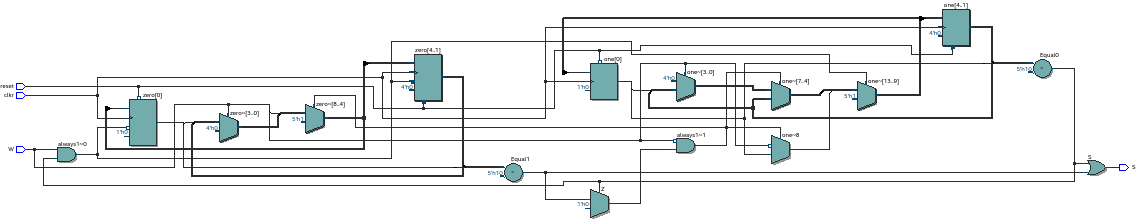
\includegraphics[scale=0.38]{fsm2reg_rtl.png}
		\caption{
			Diagrama RTL de la FSM implementada con 2 registros de corrimiento.
			\label{fig:fsm2reg_rtl}
		}
	\end{figure}
	
	\begin{figure}[ht]
		\centering
		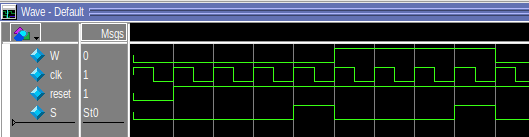
\includegraphics[scale=0.5]{fsm2reg_sim.png}
		\caption{
			Simulación de la FSM implementada con 2 registros de corrimiento.
			\label{fig:fsm2reg_sim}
		}
	\end{figure}


\enter


\subsection{Usando un registro}
	Como solo se puede utilizar un registro para el corrimiento, ya no existe la libertad de utilizar el bit de aviso para la secuencia, entonces se restringe la cantidad a 4 bits.
	
	\enter
	
	Para poder realizar las operaciones con un solo registro, se utilizan corrimientos aritméticos en lugar de lógicos. 
	En el caso de la detección de secuencia de unos, se realiza corrimiento a la 
	izquierda, mientras que para ceros, se realiza hacia la derecha.
	
	\enter
	
	Como en el inicio se arranca con alguna entrada de 1 o 0, entonces ya existe una ocurrencia antes de analizar el resto de estados, por lo que al reiniciar el conteo se coloca el detector en \texttt{1000} para 0 y \texttt{0001} para 1.
	
	\enter
	
	La salida sera 1 (secuencia detectada) cuando se complete \texttt{1111} en 
	el detector, en caso de seguir entrando 1 o 0 a la secuencia correcta y debido a que los corrimientos son de tipo aritmético, la salida conservaría su valor y por lo tanto se soportan los traslapes.
	
	\begin{figure}[ht]
		\centering
		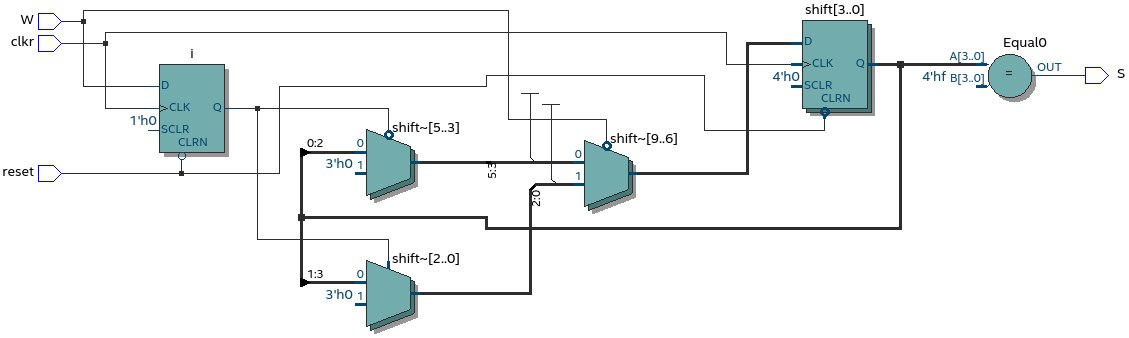
\includegraphics[scale=0.35]{fsm1reg_rtl.png}
		\caption{
			Diagrama RTL de la FSM implementada con 2 registros de corrimiento.
			\label{fig:fsm1reg_rtl}
		}
	\end{figure}
	
	\begin{figure}[ht]
		\centering
		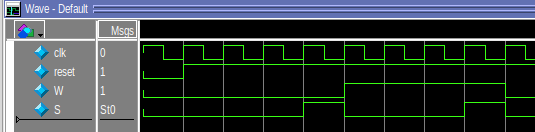
\includegraphics[scale=0.35]{fsm1reg_sim.png}
		\caption{
			Simulación de la FSM implementada con 2 registros de corrimiento.
			\label{fig:fsm1reg_sim}
		}
	\end{figure}
	
	
	
	
	
	
	
	
	
